\section{Evaluation}
\label{sec:monitoring_hard_drop.evaluation}

\subsection{Methodology} 
\label{sec:monitoring_hard_drop.evaluation.methodology}

We implemented our monitoring architecture for real-time systems by modifying
the ARM version of the gem5 simulator \cite{gem5} to support parallel hardware
monitoring and our hardware optimizations for opportunistic monitoring. In
order to explore the generality of the architecture for different monitors, we
implemented the three different monitors described in
Section~\ref{sec:monitoring_hard_drop.extensions}: uninitialized memory check
(UMC), return address check (RAC), and dynamic information flow tracking
(DIFT). We tested our system using several benchmarks from the M{\"a}lardalen
WCET benchmark suite \cite{malardalen}. 

% Size of memory structures: FIFO, MIT, MISP
We model the main and monitoring cores as 500 MHz in-order cores, each with 16
KB of L1 I/D-caches. The latency to main memory is 15 ns. This setup is
similar to Freescale's i.MX353 processor which targets embedded, automotive,
and industrial applications. For our experiments, we used a FIFO of 16 entries
connecting the main and monitoring cores. The MISP was 16 entries matching the
16 registers found in the ARM architecture. The MIT was configured with 2 ways
and 256 entries. 

% WCET
No static WCET analysis tools exist for the gem5 simulator. In order to
estimate the WCET of tasks, we ran tasks several times on the gem5 simulator
and took the worst-case observed execution time. Our WCET estimate is expected
to be lower than those that a WCET analysis tool would generate since WCET
analysis tools guarantee a conservative estimate. As a result, in our
experiments the gap between actual execution times and our estimated WCET is
lower than what we would expect with a WCET analysis tool. Therefore, the
results we present for the amount of monitoring that can be done are less than
what is expected when a strictly conservative WCET is used.

\subsection{Amount of Monitoring Performed}
\label{sec:monitoring_hard_drop.evaluation.coverage}

% Monitoring event breakdown for UMC
\begin{figure}
  \begin{center}
    \begin{subfigure}[UMC]{
      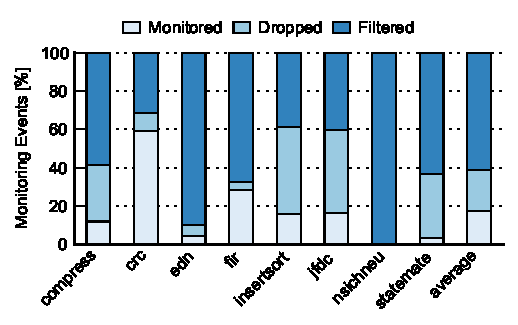
\includegraphics{monitoring_hard_drop/data/zero_slack_umc.pdf}
      \label{fig:monitoring_hard_drop.evaluation.zero_slack_umc}
    }
    \end{subfigure}

    \begin{subfigure}[RAC]{
      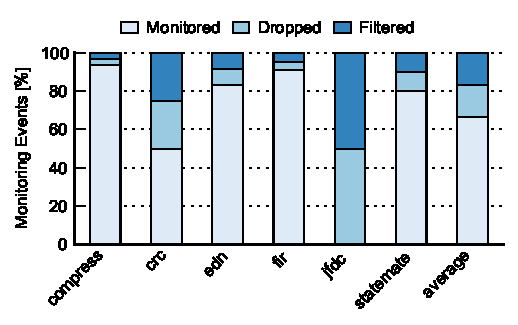
\includegraphics{monitoring_hard_drop/data/zero_slack_lrc.pdf}
      \label{fig:monitoring_hard_drop.evaluation.zero_slack_lrc}
    }
    \end{subfigure}

    \begin{subfigure}[DIFT]{
      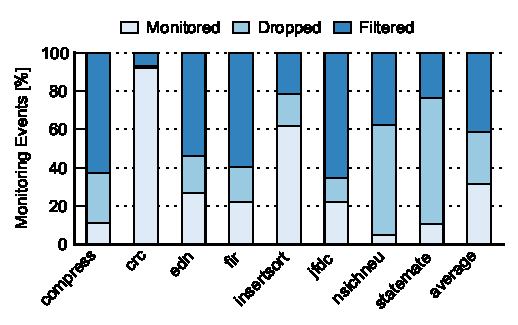
\includegraphics{monitoring_hard_drop/data/zero_slack_dift.pdf}
      \label{fig:monitoring_hard_drop.evaluation.zero_slack_dift}
    }
    \end{subfigure}

    \caption{Percentage of monitored, dropped, and filtered monitoring events
    with zero headstart slack.}
    \label{fig:monitoring_hard_drop.evaluation.zero_slack}

  \end{center}
\end{figure}

Figure~\ref{fig:monitoring_hard_drop.evaluation.zero_slack} shows the number of
monitoring events that are monitored, dropped, and filtered for UMC, RAC, and
DIFT as a percentage of the total number of monitoring events.  In these
experiments, no headstart slack was added. Thus, we see that a portion of
monitoring can still be done without exceeding the main task's original WCET.
This is due to the dynamic slack that is gained during run time. On average,
UMC (Figure~\ref{fig:monitoring_hard_drop.evaluation.zero_slack_umc}) can
perform 17\% of its monitoring tasks. RAC
(Figure~\ref{fig:monitoring_hard_drop.evaluation.zero_slack_lrc}) can perform
66\% of its monitoring and DIFT
(Figure~\ref{fig:monitoring_hard_drop.evaluation.zero_slack_dift}) can perform
31\% of its monitoring.  No results are shown for {\tt insertsort} and {\tt
nsichneu} for RAC because these benchmarks do not make any function calls.  For
DIFT, we store the actual DIFT register file metadata in the MISP instead of
invalidation flags as discussed in
Section~\ref{sec:monitoring_hard_drop.extensions.dift}.  This optimization
allows us to use the MIM and MFM to perform certain monitoring tasks. These
correct metadata updates are counted as ``Monitored'' in the statistics while
events are counted as dropped or filtered only if they were handled by the
dropping hardware due to insufficient slack.

% Coverage
\begin{figure}
  \begin{center}
    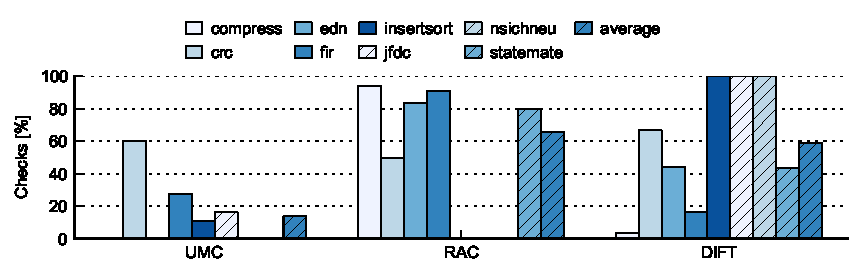
\includegraphics{monitoring_hard_drop/data/zero_slack_coverage.pdf}
    \caption{Percentage of checks that are not dropped or filtered for zero
    headstart slack.}
    \label{fig:monitoring_hard_drop.evaluation.zero_slack_coverage}
  \end{center}
\end{figure}

As expected, false positives never occurred in our experiments. However, false
negatives can occur due to dropping monitoring tasks. Specifically, dropped or
filtered check-type monitoring operations can result in false negatives.
Figure~\ref{fig:monitoring_hard_drop.evaluation.zero_slack_coverage} shows the
number of checks that are monitored as a percentage of the total checks. This
acts as a measure of the coverage achieved by the monitors. The coverage for
UMC is 15\% on average and the coverage for RAC is 66\% on average. The average
coverage for DIFT is 59\% which is much higher than the percentage of
monitoring tasks that are not dropped or filtered. In fact, for some of the
benchmarks, DIFT is able to achieve 100\% coverage. This implies that only a
portion of the monitoring operations performed by DIFT actually affect the
checks.  For example, DIFT propagates metadata on every ALU, load, and store
instruction. However, only instructions that eventually propagate metadata to
an indirect jump instruction affect the coverage.

% Coverage for UMC
\begin{figure}
  \begin{center}
    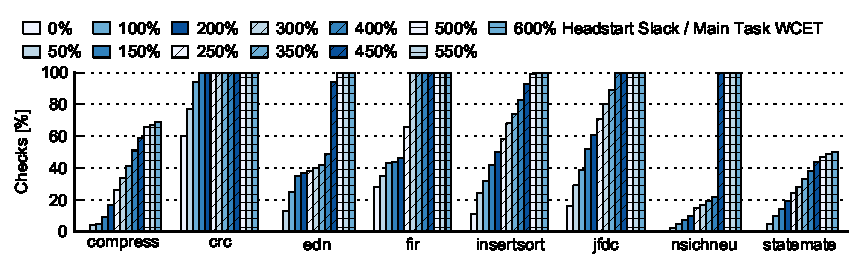
\includegraphics{monitoring_hard_drop/data/umc_sweep.pdf}
    \caption{Percentage of checks performed as headstart slack is varied for
    UMC. Headstart slack is shown normalized to the main task's WCET.}
    \label{fig:monitoring_hard_drop.evaluation.umc_sweep}
  \end{center}
\end{figure}

% Coverage for LRC
\begin{figure}
  \begin{center}
    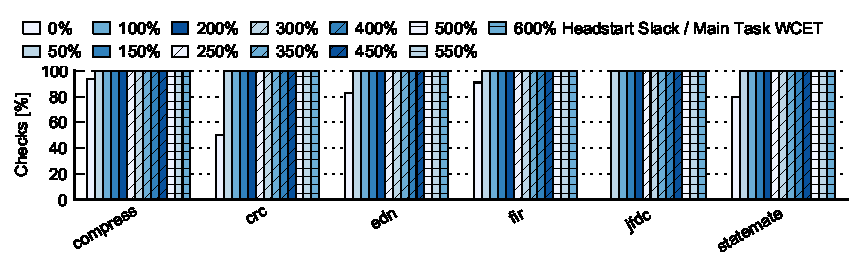
\includegraphics{monitoring_hard_drop/data/lrc_sweep.pdf}
    \caption{Percentage of checks performed as headstart slack is varied for
    RAC implemented on a processor core. Headstart slack is shown normalized
    to the main task's WCET.}
    \label{fig:monitoring_hard_drop.evaluation.lrc_sweep}
  \end{center}
\end{figure}

% Coverage DIFT
\begin{figure}
  \begin{center}
    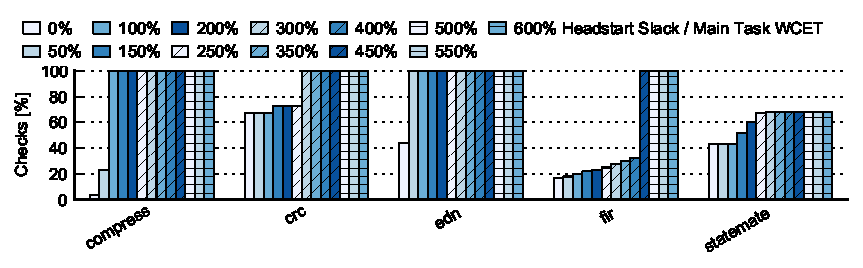
\includegraphics{monitoring_hard_drop/data/dift_sweep.pdf}
    \caption{Percentage of checks performed as headstart slack is varied for
    DIFT. Headstart slack is shown normalized to the main task's WCET.}
    \label{fig:monitoring_hard_drop.evaluation.dift_sweep}
  \end{center}
\end{figure}

For an underutilized system, if some headstart slack is given to a task
initially, then the amount of monitoring that can be performed can be
increased. As an example,
Figure~\ref{fig:monitoring_hard_drop.evaluation.umc_sweep} shows how the
coverage increases as we increase the headstart slack given to the main task
for UMC. Figure~\ref{fig:monitoring_hard_drop.evaluation.lrc_sweep} shows how
the coverage varies with headstart slack for RAC and
Figure~\ref{fig:monitoring_hard_drop.evaluation.dift_sweep} shows the coverage
variation for DIFT. The
headstart slack is displayed as a percentage of the main task's WCET for each
benchmark and is varied from 0\% to 600\%. With enough headstart slack, 100\%
of the monitoring is able to be performed. For DIFT, only benchmarks which were
not able to reach 100\% coverage with zero headstart slack are shown.  
% {\tt
% compress} and {\tt statemate} do not reach 100\% coverage across the varied
% range. This is not surprising as both had especially high WCET for performing
% monitoring without dropping (see
% Figure~\ref{fig:monitoring_hard_drop.drop.sw_drop_wcet}). With higher headstart
% slack, these benchmarks should also reach 100\% coverage.

\subsection{FPGA-based Monitor}
\label{sec:monitoring_hard_drop.evaluation.fpga}

% Monitoring event breakdown for FPGA
\begin{figure}
  \begin{center}
    \begin{subfigure}[UMC]{
      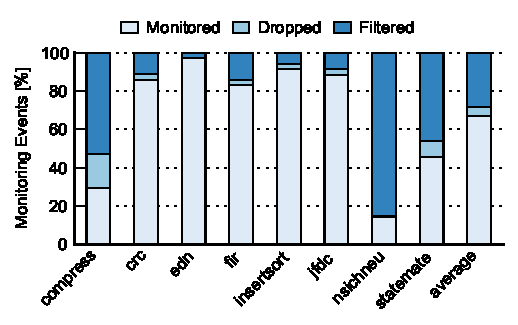
\includegraphics{monitoring_hard_drop/data/zero_slack_flex_umc.pdf}
      \label{fig:monitoring_hard_drop.evaluation.zero_slack_flex_umc}
    }
    \end{subfigure}

    \begin{subfigure}[RAC]{
      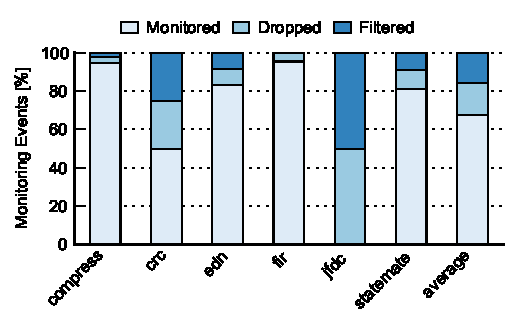
\includegraphics{monitoring_hard_drop/data/zero_slack_flex_lrc.pdf}
      \label{fig:monitoring_hard_drop.evaluation.zero_slack_flex_lrc}
    }
    \end{subfigure}

    \begin{subfigure}[DIFT]{
      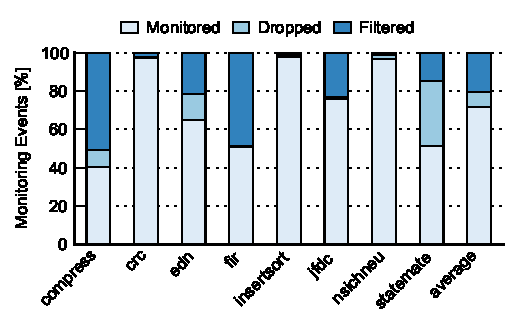
\includegraphics{monitoring_hard_drop/data/zero_slack_flex_dift.pdf}
      \label{fig:monitoring_hard_drop.evaluation.zero_slack_flex_dift}
    }
    \end{subfigure}

    \caption{Percentage of monitored, dropped, and filtered monitoring events
    for an FPGA-based monitor with zero headstart slack.}
    \label{fig:monitoring_hard_drop.evaluation.zero_slack_flex}
  \end{center}
\end{figure}

% Coverage
\begin{figure}
  \begin{center}
    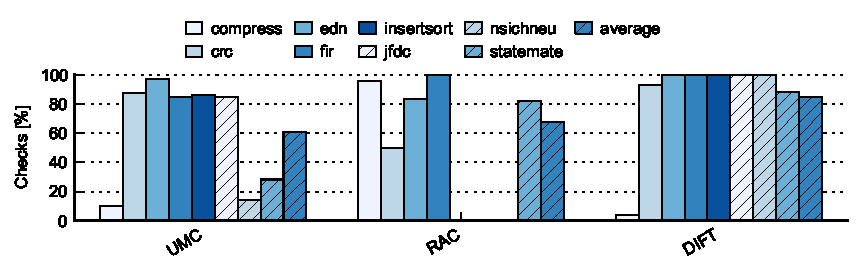
\includegraphics{monitoring_hard_drop/data/zero_slack_flex_coverage.pdf}
    \caption{Percentage of checks that are not dropped or filtered on an
    FPGA-based monitor for zero headstart slack.}
    \label{fig:monitoring_hard_drop.evaluation.zero_slack_flex_coverage}
  \end{center}
\end{figure}

Performing monitoring in software, although parallelized, can still incur high
overheads since multiple instructions are needed to handle each monitoring
event. One possible solution to improve the performance of monitoring while
maintaining programmability is to use an FPGA-based monitor
\cite{flexcore-micro10}. We model the FPGA-based monitor as being able to run
at 250 MHz and handle up to one monitoring event each cycle. Note that this
means that the FPGA-based monitor can process a monitoring event every two
cycles of the main core which runs at 500 MHz.
Figure~\ref{fig:monitoring_hard_drop.evaluation.zero_slack_flex} shows the
number of monitored, dropped, and filtered events with no headstart slack for
this FPGA-based monitor. UMC
(Figure~\ref{fig:monitoring_hard_drop.evaluation.zero_slack_flex_umc}) and RAC
(Figure~\ref{fig:monitoring_hard_drop.evaluation.zero_slack_flex_lrc}) are able
to run 67\% of their monitoring tasks on average, while DIFT
(Figure~\ref{fig:monitoring_hard_drop.evaluation.zero_slack_flex_dift}) is able
to run 72\% of its monitoring tasks on average.
Figure~\ref{fig:monitoring_hard_drop.evaluation.zero_slack_flex_coverage} shows
the coverage achieved by these monitoring schemes on an FPGA-based monitor. RAC
shows similar numbers to processor-based monitoring because the number of calls
and returns in these benchmarks is relatively small. However, for UMC and DIFT,
we see that an FPGA-based monitor allows much more monitoring to be done
without increasing the headstart slack. The coverage for UMC increases from
15\% to 62\% while the coverage for DIFT increases from 59\% to 86\%.

\begin{figure}
  \begin{center}
    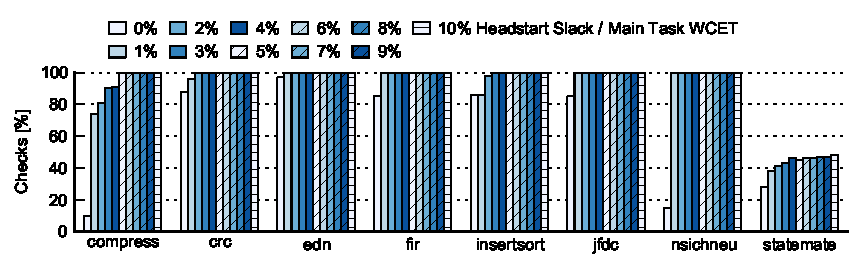
\includegraphics{monitoring_hard_drop/data/flex_umc_sweep.pdf}
    \caption{Percentage of checks performed as headstart slack is varied for
    UMC on an FPGA-based monitor. Headstart slack is shown normalized to the
    main task's WCET.}
    \label{fig:monitoring_hard_drop.evaluation.flex_umc_sweep}
  \end{center}
\end{figure}

\begin{figure}
  \begin{center}
    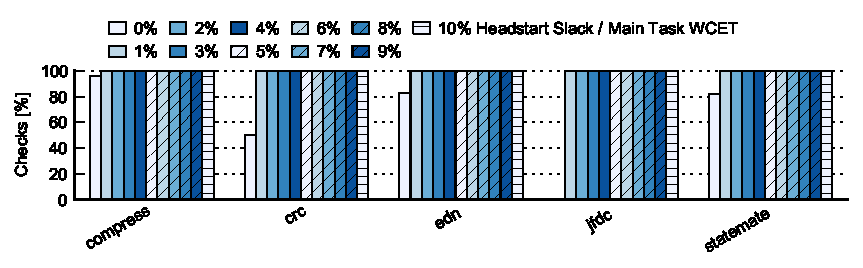
\includegraphics{monitoring_hard_drop/data/flex_lrc_sweep.pdf}
    \caption{Percentage of checks performed as headstart slack is varied for
    RAC on an FPGA-based monitor. Headstart slack is shown normalized to the
    main task's WCET.}
    \label{fig:monitoring_hard_drop.evaluation.flex_lrc_sweep}
  \end{center}
\end{figure}

\begin{figure}
  \begin{center}
    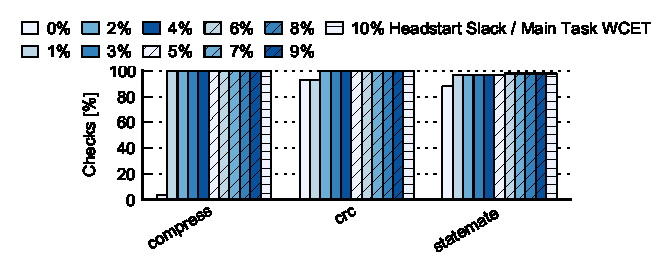
\includegraphics{monitoring_hard_drop/data/flex_dift_sweep.pdf}
    \caption{Percentage of checks performed as headstart slack is varied for
    DIFT on an FPGA-based monitor. Headstart slack is shown normalized to the
    main task's WCET.}
    \label{fig:monitoring_hard_drop.evaluation.flex_dift_sweep}
  \end{center}
\end{figure}

Figure~\ref{fig:monitoring_hard_drop.evaluation.flex_umc_sweep} shows how the
coverage for UMC varies as we increase the headstart slack from 0\% to 10\% for
an FPGA-based monitor.
Figure~\ref{fig:monitoring_hard_drop.evaluation.flex_lrc_sweep} shows this data
for RAC and Figure~\ref{fig:monitoring_hard_drop.evaluation.flex_dift_sweep}
shows this data for DIFT. Benchmark and monitoring scheme combinations which
showed 100\% coverage with zero headstart slack are omitted.  We can see that
for a high-performance FPGA-based monitor, with a small amount of slack, we are
able to achieve 100\% monitoring for almost all benchmarks while guaranteeing
the main task's execution time does not exceed its WCET. 

\subsection{Area and Power Overheads}

% Area and Power Overheads
\begin{table}[tb]
  \begin{center}
    \caption{Average power overheads for dropping hardware at zero headstart
    slack. Percentages in parentheses are normalized to the main core's power usage.}
    \begin{footnotesize}
    
% Full monitoring at zero slack

\begin{tabular}{|c|c|c|c|}
\hline

\multicolumn{2}{|c|}{\bf Monitor} & {\bf Peak Power [mW]} & {\bf Runtime Power [mW]} \\ \hline\hline

\multirow{3}{*}{Processor} 
& UMC  & 4.9 (3.2\%) & 4.7 (6.6\%) \\ \cline{2-4}
& RAC  & 4.7 (3.1\%) & 4.7 (6.6\%) \\ \cline{2-4}
& DIFT & 5.0 (3.3\%) & 4.8 (6.7\%) \\ \hline\hline

\multirow{3}{*}{FPGA} 
& UMC  & 16.7 (10.9\%) & 8.5 (11.9\%) \\ \cline{2-4}
& RAC  &  4.7  (3.1\%) & 4.7  (6.6\%) \\ \cline{2-4}
& DIFT & 13.0  (8.5\%) & 8.8 (12.3\%) \\ \hline

\end{tabular}

    \end{footnotesize}
    \label{tab:monitoring_hard_drop.evaluation.area_power}
  \end{center}
\end{table}

Adding the dropping hardware in order to enable adjustable overheads adds
overheads in terms of area and power. We use McPAT \cite{mcpat-micro09} to get
a first-order estimate of these area and power overheads in a 40 nm technology
node. McPAT estimates the main core area as 1.96 mm$^2$ and the peak power
usage as 152.9 mW averaged across all benchmarks. The average runtime power
usage was 71.6 mW. These area and power numbers consist of the core and L1
cache, but do not include memory controllers and other peripherals. The power
numbers include dynamic as well as static (leakage) power. For the dropping
hardware, the ALUs, MISP, MIT, and configuration tables are modeled using the
corresponding objects in McPAT. We note that this is only a rough area and
power result since components such as the wires connecting these modules have
not been modeled. However, this gives a sense of the order-of-magnitude
overheads involved with implementing our approach.

An additional 0.132 mm$^2$ of silicon area is needed, an increase of 7\% of the
main core area. Table~\ref{tab:monitoring_hard_drop.evaluation.area_power}
shows the peak and runtime power overheads with zero headstart slack for both a
processor-based monitor as well as an FPGA-based monitor. The peak power is
5-17 mW, which is 3-11\% of the main core's peak power usage. The average
runtime power is 5-9 mW, corresponding to 7-12\% of the main core's runtime
power. For UMC and DIFT, the dropping hardware has lower power usage with the
processor-based monitor due to
more monitoring events being filtered out that do not require invalidation.
This reduces the activity of the Metadata Invalidation Module which reduces the
power usage.

